\documentclass{custom_report}
\usepackage{pdfpages}
\usepackage{mathptmx}

\begin{document}

\title{How does campaign financing effect the ambiguity of US state bills ?}
\author{Simon Schaefer \\ Prof. Eliot Ash (ETH Z{\"u}rich) \\ Prof. Matia Vannoni (King's College)}
\date{August 2019}

\maketitle

%=================================================================================
% ABSTRACT
%=================================================================================
\begin{abstract}
This work analyzes the impact of campaign contributions on the ambiguity of US state law. Therefore an ambiguity score for each state bill is determined using a word-sense-disambiguation and sense-similarity based algorithm and compared to the campaign contribution limits of each US state. While a correlation between the ambiguity of the analyzed bills and the campaign contribution limits can be shown, it is not large, neither varying much between different states nor industry sectors the bills are clustered to.
\end{abstract}

\maketitle
\tableofcontents

% ================================================================================
% INTRODUCTION
%=================================================================================
\chapter{Introduction}
\label{cha:introduction}
% reset page numbering.
\pagenumbering{arabic}

Lobbying has an impact on the legislation in modern democracies. One common type of lobbyism is the financial contribution to party's campaign such as in the US presidential election. According to the Washington Post about 2.3 billion US dollars have been raised in the US presidential election campaign\footnote{https://www.washingtonpost.com/graphics/politics/2016-election/campaign-finance/}. As shown in Figure \ref{fig:us_presidential} the campaign contributions are growing, and a large part are raised from companies in the financial, technical and natural resources sector, according to FED. The Campaign Financing Capture Index, that was created by the University of Chicago Booth School of Business, ranks the concentration of funding for each candidate with an eye toward predicting how political donations could influence policy decisions under a new president and measured a record concentration of political donors in Cruz campaign during the last US presidential election  \footnote{https://news.chicagobooth.edu/about/newsroom/press-releases/2016/2016-02-04}. 

\begin{figure}[h!]
\begin{center}
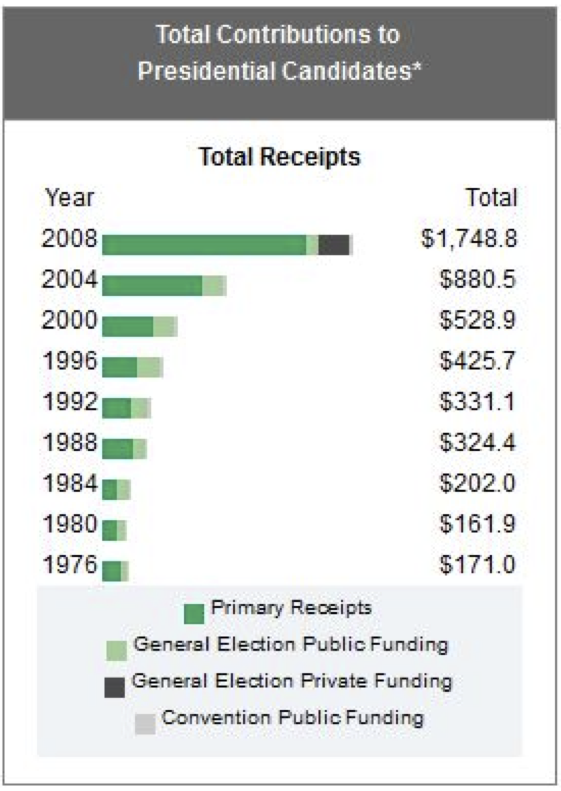
\includegraphics[height=7cm]{images/us_presidential_contribs_over_years.png}
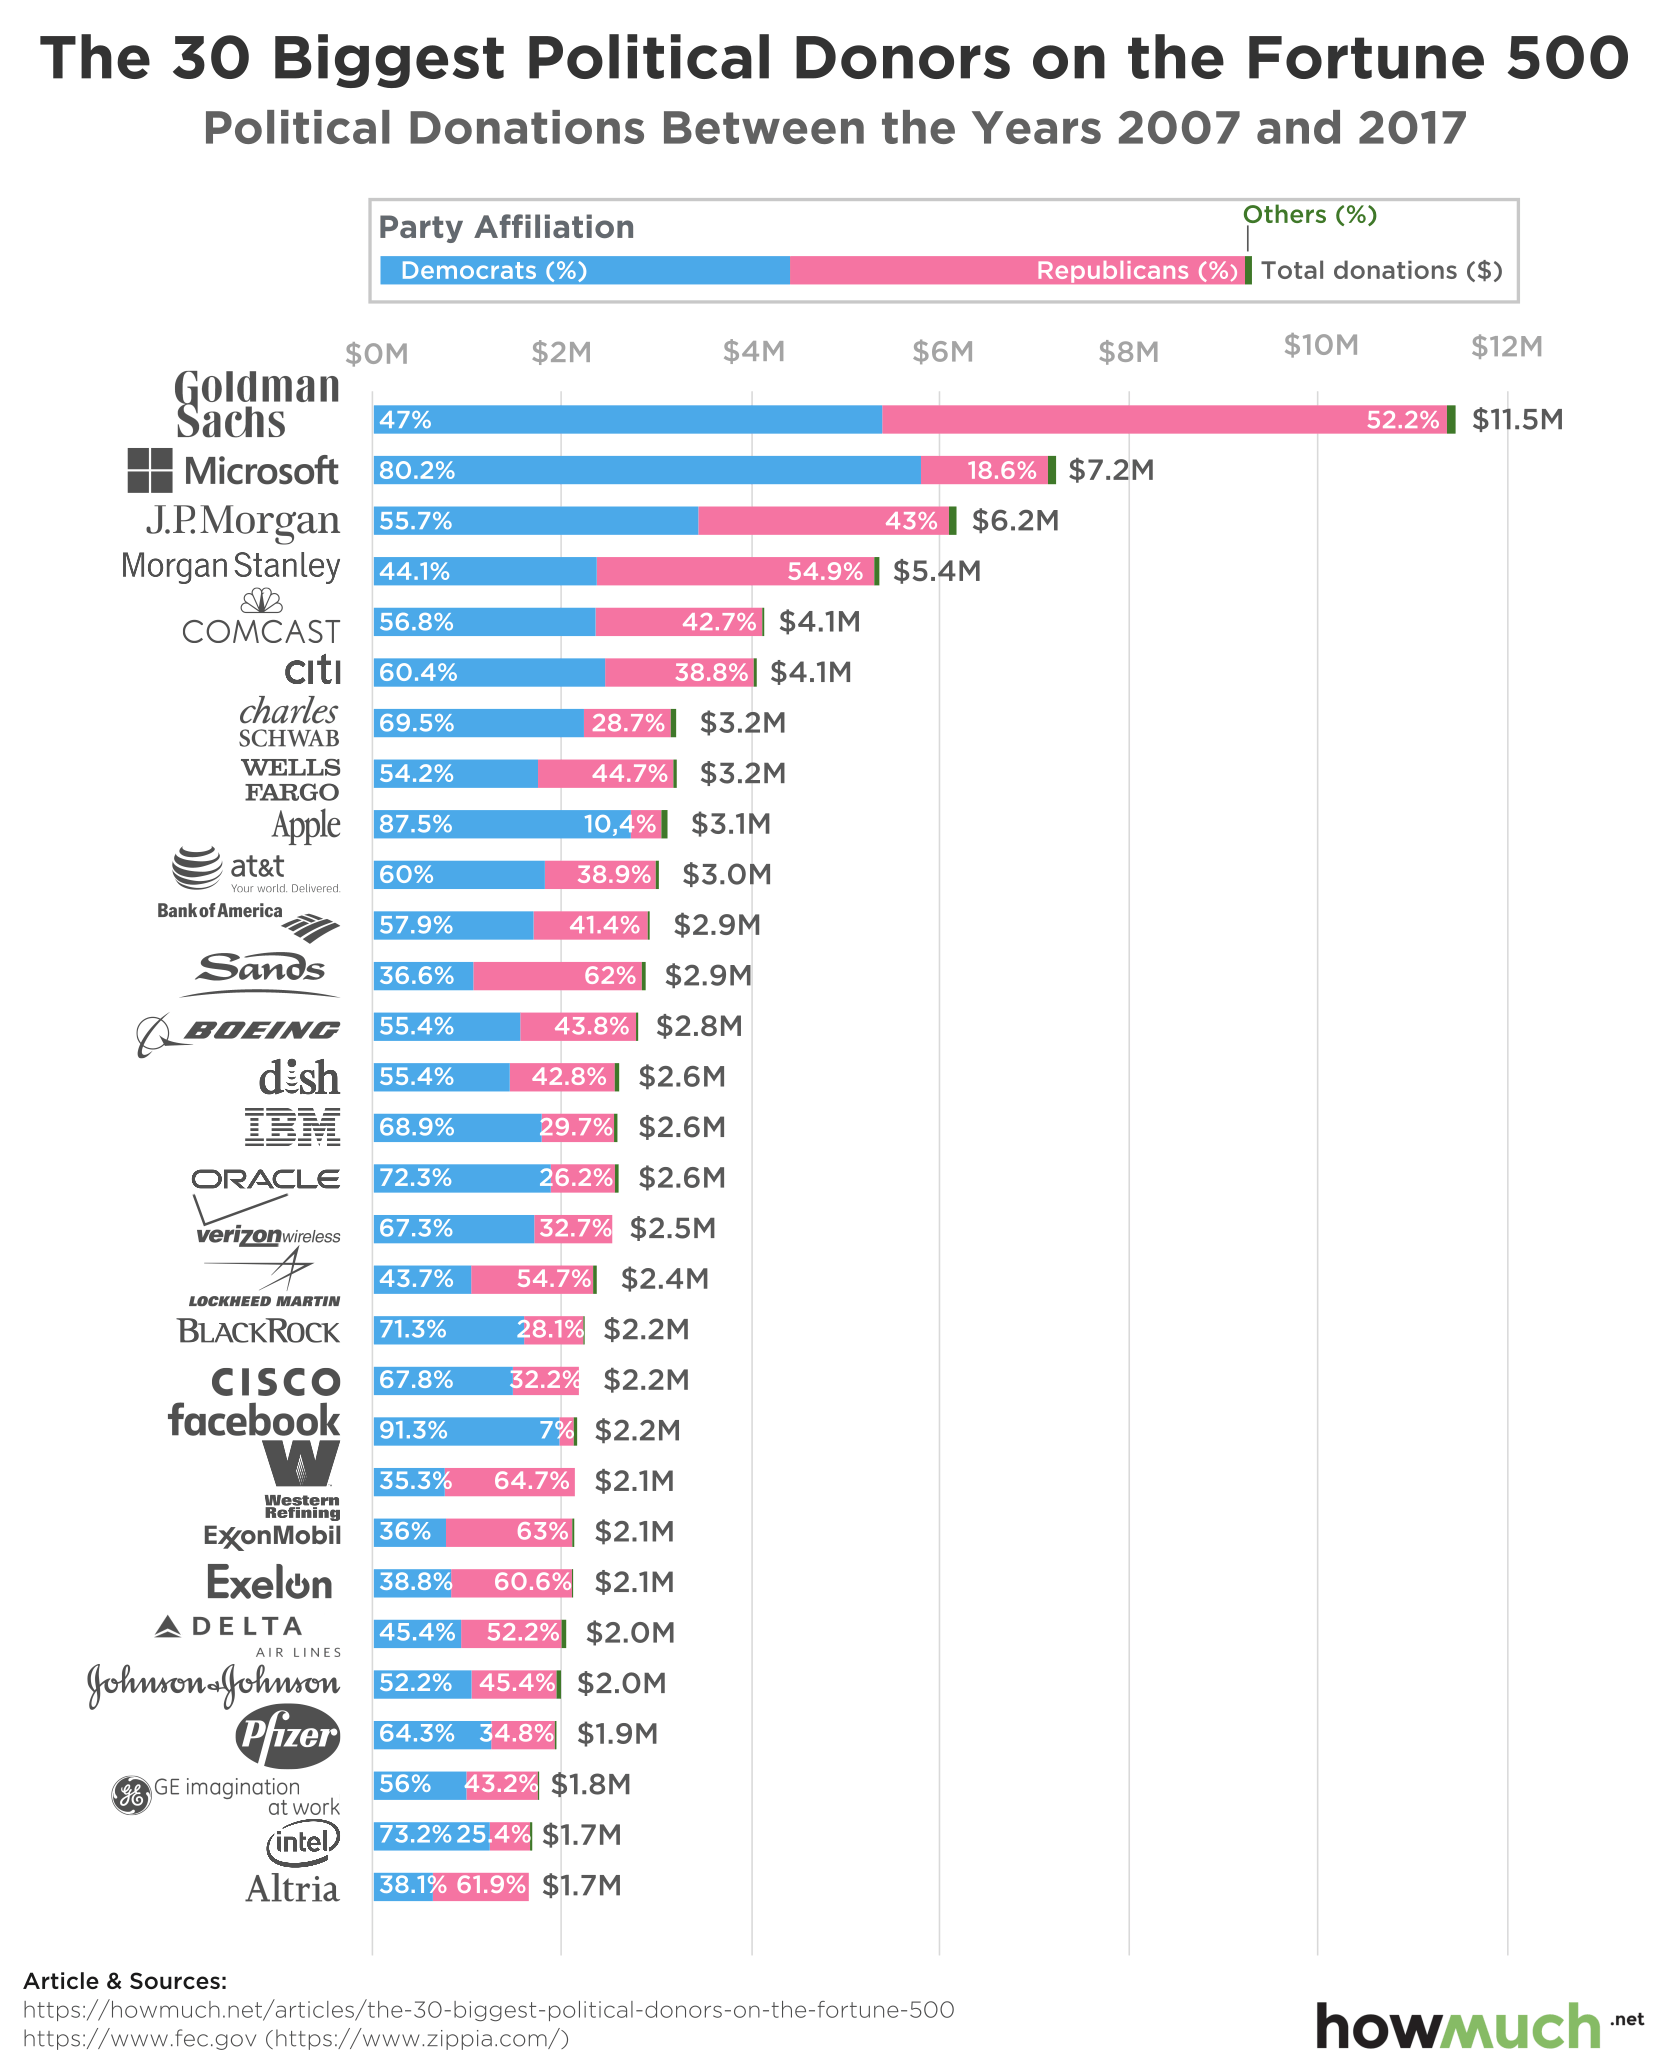
\includegraphics[height=7cm]{images/trump_vs_hillary_donors.png}
\end{center}
\caption{Development of contributions to presidential candidates (left) and biggest donors according to FED}
\label{fig:us_presidential}
\end{figure}

However although the qualitative effect of lobbying on politics meets qualitatively approval, a quantitative analysis on how much it effects the resolved bills is hardly analyzed. Therefore the goal of the underlying project is to measure the impact of lobbyism on the ambiguity of US state bills, at the example of campaign financial contributions.

% ================================================================================
% RELATED WORK
%=================================================================================
\chapter{Related Work}
\label{cha:related_work}
The impact of campaign financing has widely been discussed in recent work. However most of the work focused on the analyzing the connection between campaign contribution and electoral performance, such as \cite{brazil_campaign_finance} that ascertains a positive and statistically significant association between political finance and electoral performance in Brazil,  \cite{congressional_elections} that evaluate the impact of campaign spending on the voters behaviour in the US or \cite{social_media} studying the effect of social media such as Facebook or Twitter on the elector's spending using an unsupervised learning approach to cluster themes in candidate content. Besides, the effect of campaign finance spending bans on the electoral performance has been analyzed, concluding a merely little impact \cite{citizens_united}. 
\newline
Ambiguity has been posed as a problem of language-driven law, as Schane describes, "Law is a profession of words" in \cite{ambiguity_law_schane}. Poscher pictures that "significant portions of the institutional legal system, especially courts at the appellate level and supreme courts, are for the most part concerned not with disentangling the facts of cases but with the indeterminacies of the law" and divides ambiguity in the four categories, logic, ontology, epistemology, and semantics \cite{ambiguity_law_poscher}.  
\newline
In natural language processing ambiguity has first been tackled using word embeddings. However, word embeddings have been shown to be unable to capture different meanings of a word, even if the meaning occurs in the same dataset. In fact different meanings have a negative impact on accurate semantic modeling as unrelated words that have a sense similar to different senses of the same word are pulled together. This problem can be solved by using sense embeddings instead, associating each word a category, so that words can be distinguished as being words of the same category (hypernymys) or of different categories. As \cite{word_to_sense_embedding} describes to construct sense embeddings there are two main paradigms, unsupervised and knowledge-based models. While unsupervised models (e.g. \cite{unsupervised_latent_vector_weighting}) induce different senses of a word by analysing its contextual semantics in a corpus, knowledge-based systems such as WordNet \cite{wordnet} are based on human-inputted senses of a word. As purposed by Pilehvar and Collier \cite{knowledge_based_page_rank}, DeConf, a personalized PageRank algorithm can be used to extend word embeddings by different senses (\textit{sense biasing words}), in order to maintain the euclidean order of the embedded space (deflation problem).
\newline
So whilst different parts of the analysis of the impact of campaign contributions on the ambiguity of bills have been studied, such as ambiguity in law in general or the effect of campaign contributions, to the best of my knowledge, I am the first one connecting these areas to a single analysis. 

%=================================================================================
% APPROACH
%=================================================================================
\chapter{Approach}
\label{cha:approach}
The ambiguity of a bill text is the weighted mean of the scalar ambiguity score that is determined for each of the bill's sentences. In order to compare different industry sectors in terms of their campaign distribution's impact the bills are first separated by sector. The ambiguity of a sentence is evaluated by using word-sense-disambiguation, similarly to the approach used in \cite{word_to_sense_embedding}, i.e. the set of possible senses of the noun of the sentence is determined given its context words and summed using the similarity of the senses in the set of possible senses.

\begin{figure}[h!]
\begin{center}
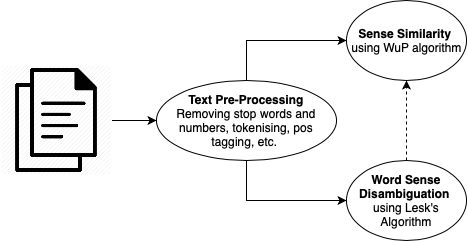
\includegraphics[width=10cm]{images/ambiguity.png}
\end{center}
\caption{Ambiguity evaluation pipeline}
\end{figure}

\section{Topic Modelling}
For the sake of simplicity and efficiency to sort the bill texts by industry sector a keyword differentiation algorithm is used. Therefore the text is tokenized and compared with predefined sets of keywords specific for each industry sector.

\begin{lstlisting}[language=Python, caption=Predefined set of keywords by industry sector, captionpos=b, basicstyle=\small]
# resources sector
"oil", "petroleum", "gas", "forest", "minerals", "minerals", "coal", "mining",
"mines", "energy", "natural gas", "fuel", "reserves", "bcl", "drilling",
"upstream", "downstream"

# agriculture sector
"farm", "rural", "agriculture", "organic", "food", "biological", "farming",
"meat", "beef", "slaugtherer", "butcher", "cow", "pork", "chicken", "rind",
"potatoes", "corn", "i rrigation", "watering", "environment", "nature",
"pollution", "pesticide", "fertilizer", "seed", "seeds"

# finance sector
"insurance", "bank", "stock market", "stock exchange", "leasing", "finance",
"investing", "investemont", "asset", "assets", "deposit", "deposits", "fund",
"funds", "money", "market", "crisis", "management", "mortgage"
\end{lstlisting}

\section{Ambiguity Score}
For ambiguity analysis the word-sense-ambiguation using Lesk's algorithm \cite{lesk} is used, which basically compares the context of a word with its dictionary definitions, assuming that words in the queried neighbourhood share a common topic. Since bills usually are written in a dense manner and specifically targeting a topic this condition is assumed to be met within the project.

\subsection{Word-Sense-Disambiguation}
In order to explain Lesk's algorithm consider the following (standard) example sentence:

\vspace*{0.5cm}
\begin{center}
\textit{I went to the bank to deposit money.}
\end{center}
\vspace*{0.5cm}

while the ambiguity of the word \textit{bank} should be inferred, given its context words. Since stop words such as \textit{to} or \textit{the} do not contain context information they are removed in the first step. Afterwards NLTK's wordnet \cite{wordnet} is queried to determine every sense of the target word (\textit{bank}), and compared to the given contextual information. In the example above the word \textit{bank} has the 16 different senses such as the financial institution, the bank as a building, the money container, sloping land next to a body of water, but also verbs such as having confidence in something or someone. The whole list of different senses is shown in the following: 

\begin{lstlisting}[language=Python, caption=Predefined set of keywords by industry sector, captionpos=b, basicstyle=\small]
- 'sloping land (especially the slope beside a body of water)',
- 'a financial institution that accepts deposits and channels the money into lending activities',
- 'a long ridge or pile',
- 'an arrangement of similar objects in a row or in tiers',
- 'a supply or stock held in reserve for future use (especially in emergencies)',
- 'the funds held by a gambling house or the dealer in some gambling games',
- 'a slope in the turn of a road or track; the outside is higher than the inside in order to reduce the effects of centrifugal force',
- 'a container (usually with a slot in the top) for keeping money at home',
- 'a building in which the business of banking transacted',
- 'a flight maneuver; aircraft tips laterally about its longitudinal axis (especially in turning)',
- 'tip laterally',
- 'enclose with a bank',
- 'do business with a bank or keep an account at a bank',
- 'act as the banker in a game or in gambling',
- 'be in the banking business', 'put into a bank account',
- 'cover with ashes so to control the rate of burning',
- 'have confidence or faith in'
\end{lstlisting}

In order to figure out the actual sense of the queried word its context is compared to the different sense definitions, the more key words match the more likely it is that the queried word's meaning can be determined un-ambiguously. 

\subsection{Sense Similarity}
However there are many queries returning multiple possible matches, since the keywords of multiple sense definitions occur in the context of the queried word. In this case two scenarios are possible, either the queried word actually is ambiguous or multiple senses can be assigned but these senses in fact are similar, so that the ambiguity of the queried word is low. To distinguish these different cases automatically the similarity measure between the assigned senses is determined and combined with the matching score for each assigned sense. 
\newline 
Most efficient similarity measures are based on a hierarchical sense taxonomy structure like WordNet \cite{wordnet}, stating that word senses are generally less similar the longer the path distance between them in the taxonomy graph is, i.e. the more edges are between them \cite{speech_and_language_processing}. The simplest similarity metric (path-similarity) therefore is determined by the number of edges between the queried sense nodes in the taxonomy graph, scaled by a maximum distance. Due to linearity of the distribution of similarity scores obtained by using path similarity is very skewed to small scores, therefore it is re-scaled using negative logarithm in Leacock-Chodorow (LCH) \cite{lch_similarity}.
\newline 
The Wu-Palmer (WuP) metric \cite{wup_similarity} additionally weights the counted edges based on the depth in the taxonomy graph hierarchy, attaching more weight on type changing operations the higher in the hierarchy they are \cite{speech_and_language_processing}, thereby normalizing the final similarity score. Transferred to the Edit distance between two words \cite{edit_distance} the WuP-similarity would weight a change from \textit{weight} to \textit{eight} much larger than changing from \textit{alike} to \textit{like}, since the former change occurs a lot higher in the taxonomy graph, although the Edit distance is the same in both transitions.  
\newline 
More advanced methods such as Resnik \cite{resnik_similarity} or Jiang-Conrath-similarity \cite{jiang_similarity} also the take the information content (IC) of the lowest common subsumer between the two sense nodes into account, instead of merely comparing (weighted) distances between them \cite{nltk}. However, although IC-based methods have shown to work better then the purely graph-based methods (e.g. LCH, WuP) they are specific to the database the information content is sampled from \cite{speech_and_language_processing}. On the other side the text which is analyzed within the project is fairly general, not domain specific. Also graph-only based methods are a lot more efficient, in terms of computational complexity. For these reasons the WuP-similarity is used. 

\subsection{Combining sense and similarity scores}
By applying word-sense-disambiguation and sense similarity metrics a vector of $N$ non-zero sense scores $w_S$ and a $NxN$ matrix containing similarity scores $Z$ is obtained. To ascertain the final ambiguity of a queried word given its context both are combined by multiplying the adjoint of the similarity matrix with the sense score vector, the actual ambiguity score then is the ratio between the maximum value of the resulting vector divided by the sum of all its elements: 

\begin{align*}
S = adj(Z) = ||Z|| \cdot Z^{-1} \\
Ambiguity\_Score = \epsilon  = \frac{(S \cdot w_S)_{min}}{\sum S_i {w_S}_i}
\end{align*}

The adjunct is built by the sub-determinants of each matrix element, i.e. figuratively spoken the determinant of the matrix resulting when the row and column of the matrix element are erased. In this context the adjunct of the similarity matrix can be understood as the accumulated similarity score of the remaining senses if one sense is deleted. The max-sum ratio then takes into account the distribution of the sense scores, e.g. whether the distribution is uniformly or skewed to one sense.
\newline
As an example consider the 3-sense vector $w_S = [a, b, c]^T$ with general scores $a$, $b$ and $c$; and the following similarity matrices $Z_{ij} = wup\_similarity(sense_i, sense_j)$: 

$$Z_1 = \begin{bmatrix} 1 0 0 \\ 0 1 0 \\ 0 0 1\end{bmatrix} Z_2 = \begin{bmatrix} 1 1 1 \\ 1 1 1 \\ 1 1 1\end{bmatrix} Z_3 = \begin{bmatrix} 1 1 0 \\ 1 1 0 \\ 0 0 1\end{bmatrix}$$

so that in $Z_1$ the three senses are totally independent, in $Z_2$ totally similar and two senses are similar while one of them is independent in $Z_3$. A trivial multiplication $S = Z \cdot w_S$ would result in the same ambiguity score for the first and the second scenario, assuming a uniform distribution of sense scores ($a = b = c$), although the first scenario is highly ambiguous (three independent senses) while the second scenario is not (three similar senses). For the reasons explained above using the adjunct of $Z$ instead results in the ambiguity scores such as $\epsilon_2 = 0$ and $\epsilon_3 = 0.5$, as expected, again assuming a uniform distribution of sense scores. Also if the sense score distribution is highly skewed to one sense (e.g. $c >> a + b$) then the final ambiguity score decreases, since they are more hints for assigning one sense then other senses, e.g. for $w_S = [1, 1, 10]$ and $Z = Z_1$ we get $\epsilon_1 = 0.08$. 
\newline
Referring to the example sentence above the two distinguished senses of \textit{bank}, bank as financial institution and the actual building, are quite non-similar, using WuP-similarity, since the on sense belongs to the group economical entities and the other one to buildings and houses. Therefore a large ambiguity score is obtained. 

\vspace*{0.5cm}
\begin{center}
\textit{The river overflowed the bank, everything is under water.}
\end{center}
\vspace*{0.5cm}

The sentence above is another example of a context the word \textit{bank} could be in. Here only one sense, the \textit{bank} as sloping land is inferred, resulting in an ambiguity score equal to zero. 

\section{Other text features}
Other than the ambiguity estimation itself several features are extracted from each text, as a reference value for the ambiguity score. From human intuition a bill is percepted as more being more factfulness and exact with growing number of descriptives such as adjectives or numbers in the text.\footnote{This is just a claim from personal insight, but still can be used for the matters of comparison to the actual ambiguity score.}\footnote{In order to not take dates of commencement or other non-bill-content related numbers into account, all dates are removed.} Therefore there might be a correlation between the ambiguity on the one and the number of these descriptives on the other side. Since these numbers can be determined efficiently after tokenisation they are also extracted from the bills text, normalized by the total number of tokens contained in each bill.  
\newline 
A similar arguments holds for the length of the bill. Especially due to the dense format bills usually are formulated with a longer, the bill's ambiguity might be inversely correlated with the bill's length, since more details can be specified. Accordingly, a comparably short bill as the first article of the constitution of Germany, "The integrity of the human is inviolable", without any additions can be qualified as highly ambiguous since the definition and extent of \textit{integrity} is not given. For this reason the length of the bill, i.e. the number of non-stop-words and non-punctuation tokens, is extracted from the bill's text as well. 

%=================================================================================
% EXPERIMENTS AND RESULTS
%=================================================================================
\chapter{Experiments and Results}
\label{cha:exp_and_results}
The described approach is applied to evaluate the correlation between US state campaign contributions and the ambiguity in its bills. All experiments are implemented in Python3, primarily using the nltk natural language processing framework \cite{nltk}. 

\section{Datasets}
Therefore two datasets are used, the US statue dataset from E. Ash and the US campaign contribution dataset by E. Ash and M. Vannoni. 

\subsection{US campaign contributions}
The US campaign contributions dataset summarizes the state election campaign contribution limits in each US state from 1951 to 1999, by assigning one of the categories \textit{unlimited}, \textit{individual} and \textit{restricted}. Figure \ref{fig:usc_grid} shows the labels given in the dataset per state and year, while non-given data points are given the label \textit{undefined}. Figure \ref{fig:usc_map} displays the contribution limits in 1999 by state.  

\begin{figure}[h!]
\begin{center}
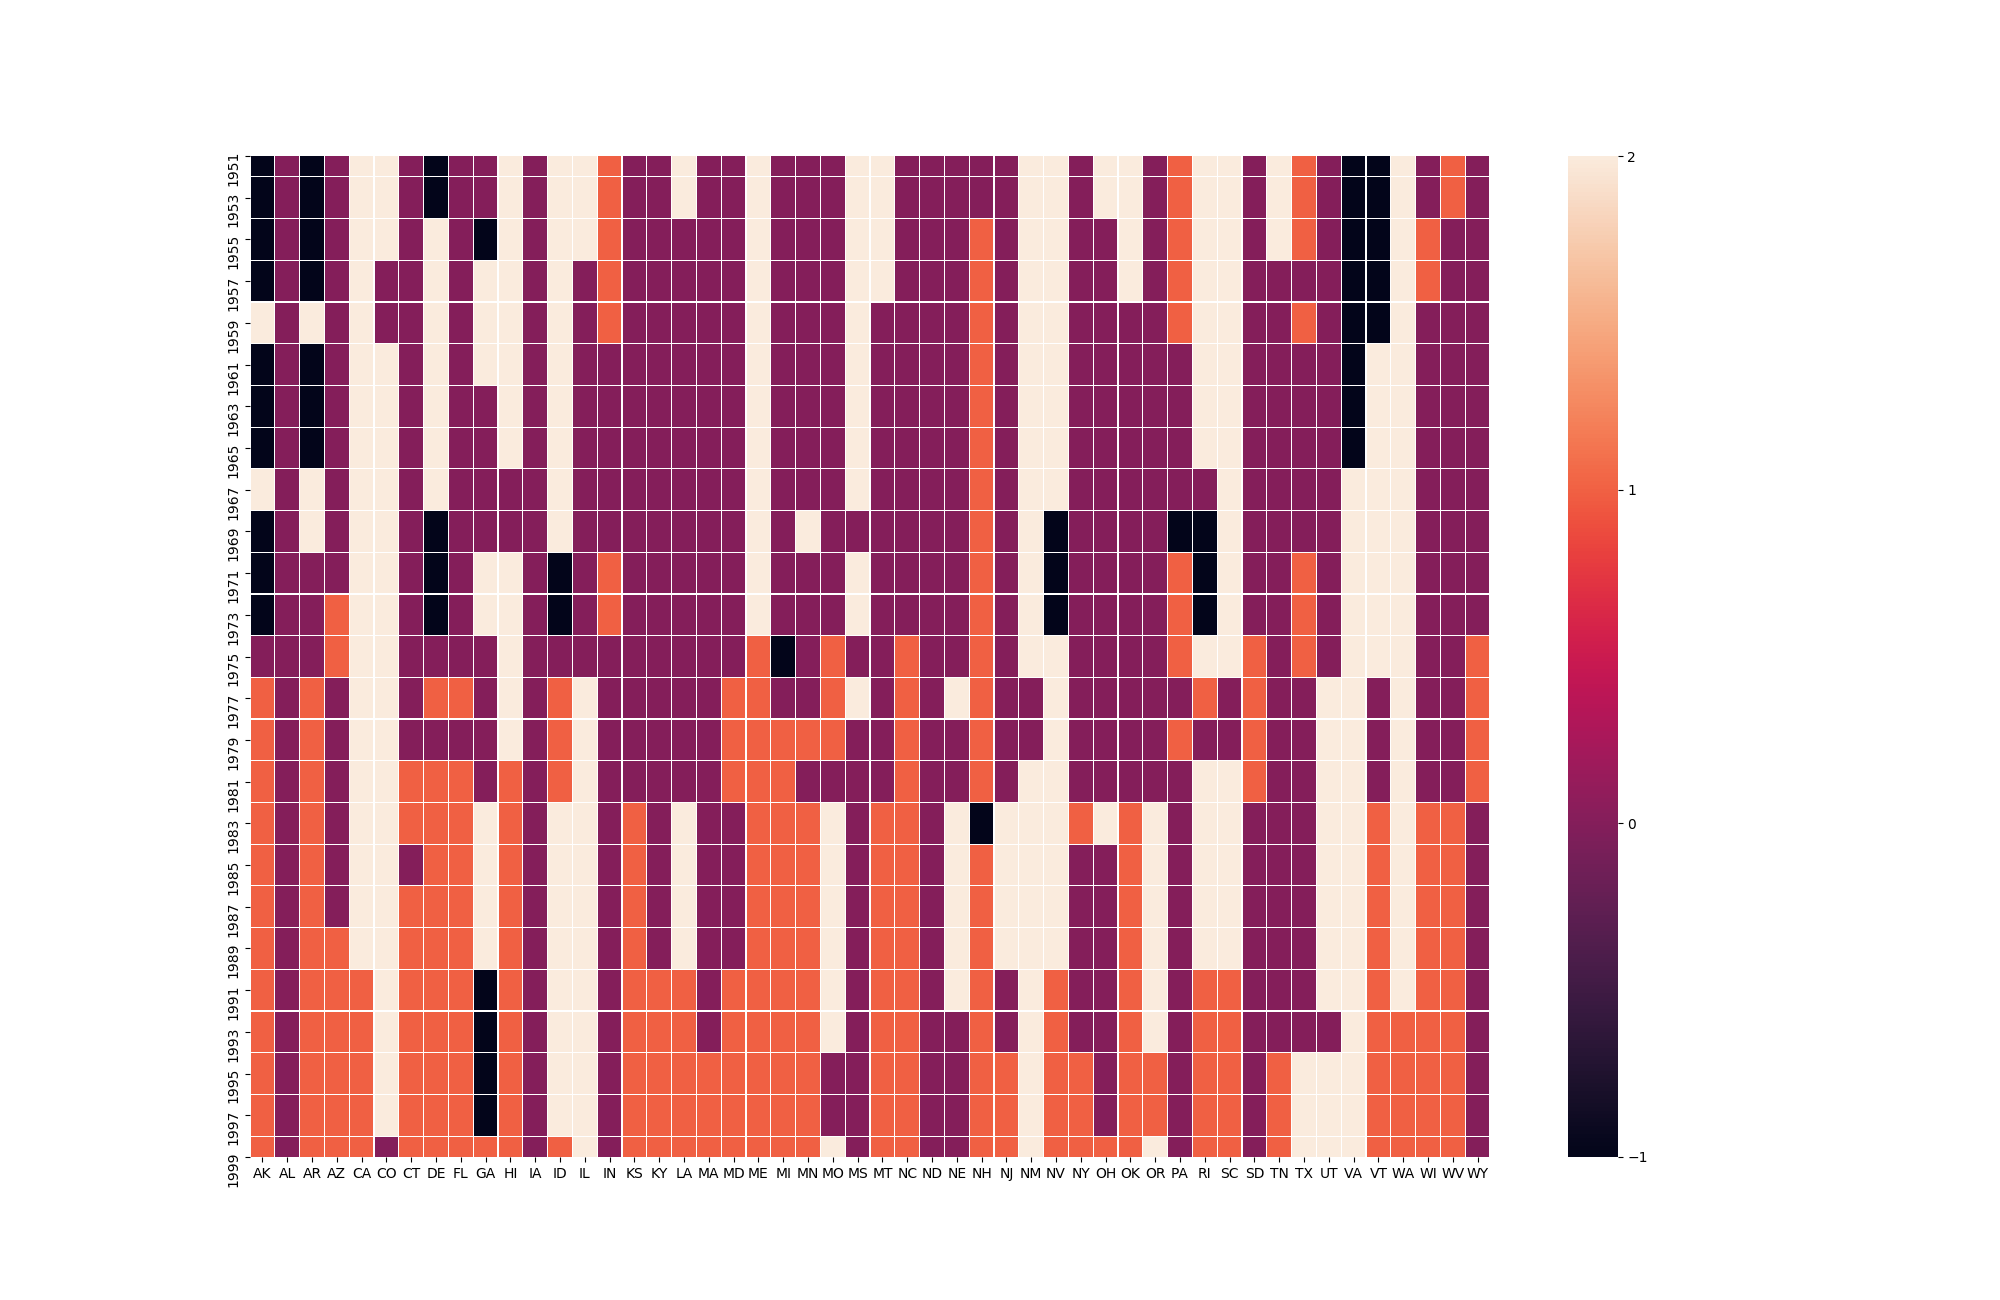
\includegraphics[width=12cm]{images/usc_state_years.png}
\end{center}
\caption{US campaign contributions by state and year: -1 = \textit{undefined}, 0 = \textit{unlimited}, 1 = \textit{individual}, 2 = \textit{restricted}}
\label{fig:usc_grid}
\end{figure}

\subsection{US state statues}
The US statue dataset contains bills for every US state voted upon in the time period from 1950 until recently, stating next to the bill's text several information about the formation and voting process, formatted in HTML markup. Thereby each document includes information about the state, the year, the member of parliament that brought the bill proposal in and several other details and the bill's text itself, whereby several ten-thousands of documents are assigned to each state (e.g. about $150000$ documents to the state New York). 

\section{Evaluation workflow}
Figure \ref{fig:workflow} shows the overall workflow of the evaluation. The bills in the US statue dataset are parsed and preprocessed (stop words and numericals removal, tokenization, pos tagging). Afterwards word-sense-ambiguation and sense similarity analysis are applied as described in chapter \ref{cha:approach} as well as text features are extracted. Thereby the ambiguity score of every noun in the bill's text is determined, because it both simplifies word-sense-disambiguation as the function of the queried word in the sentence is known and is applicable to whole text. The final ambiguity score, being the mean of all ambiguity scores in all documents which are assigned to a state, is compared to the state's contribution limits.

\begin{figure}[h!]
\begin{center}
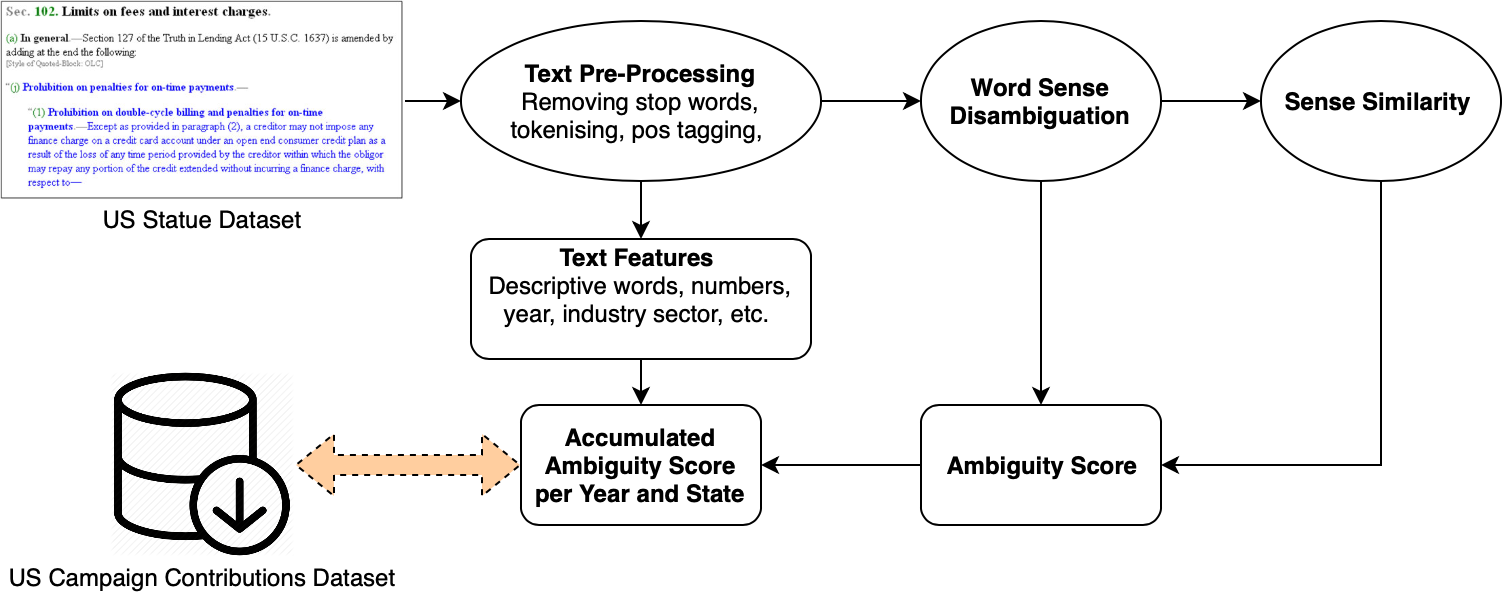
\includegraphics[width=12cm]{images/workflow.png}
\end{center}
\caption{Experiment workflow using US statue and campaign contribution dataset}
\label{fig:workflow}
\end{figure}

\section{Results}
Figure \ref{fig:uss_ambiguity_by_state} displays the distribution of ambiguity scores over all sectors and years from 1950, divided by US state. As shown are the distributions over states very close to each other, e.g. the median value is minimal in Indiana about $0.30$ and maximal in New Mexico about $0.38$, meaning that most of the occurring ambiguities are two-senses-based, i.e. can be assigned to two widely independent senses with similar scores, while one of the senses is slightly more probable. 

\begin{figure}[h!]
\begin{center}
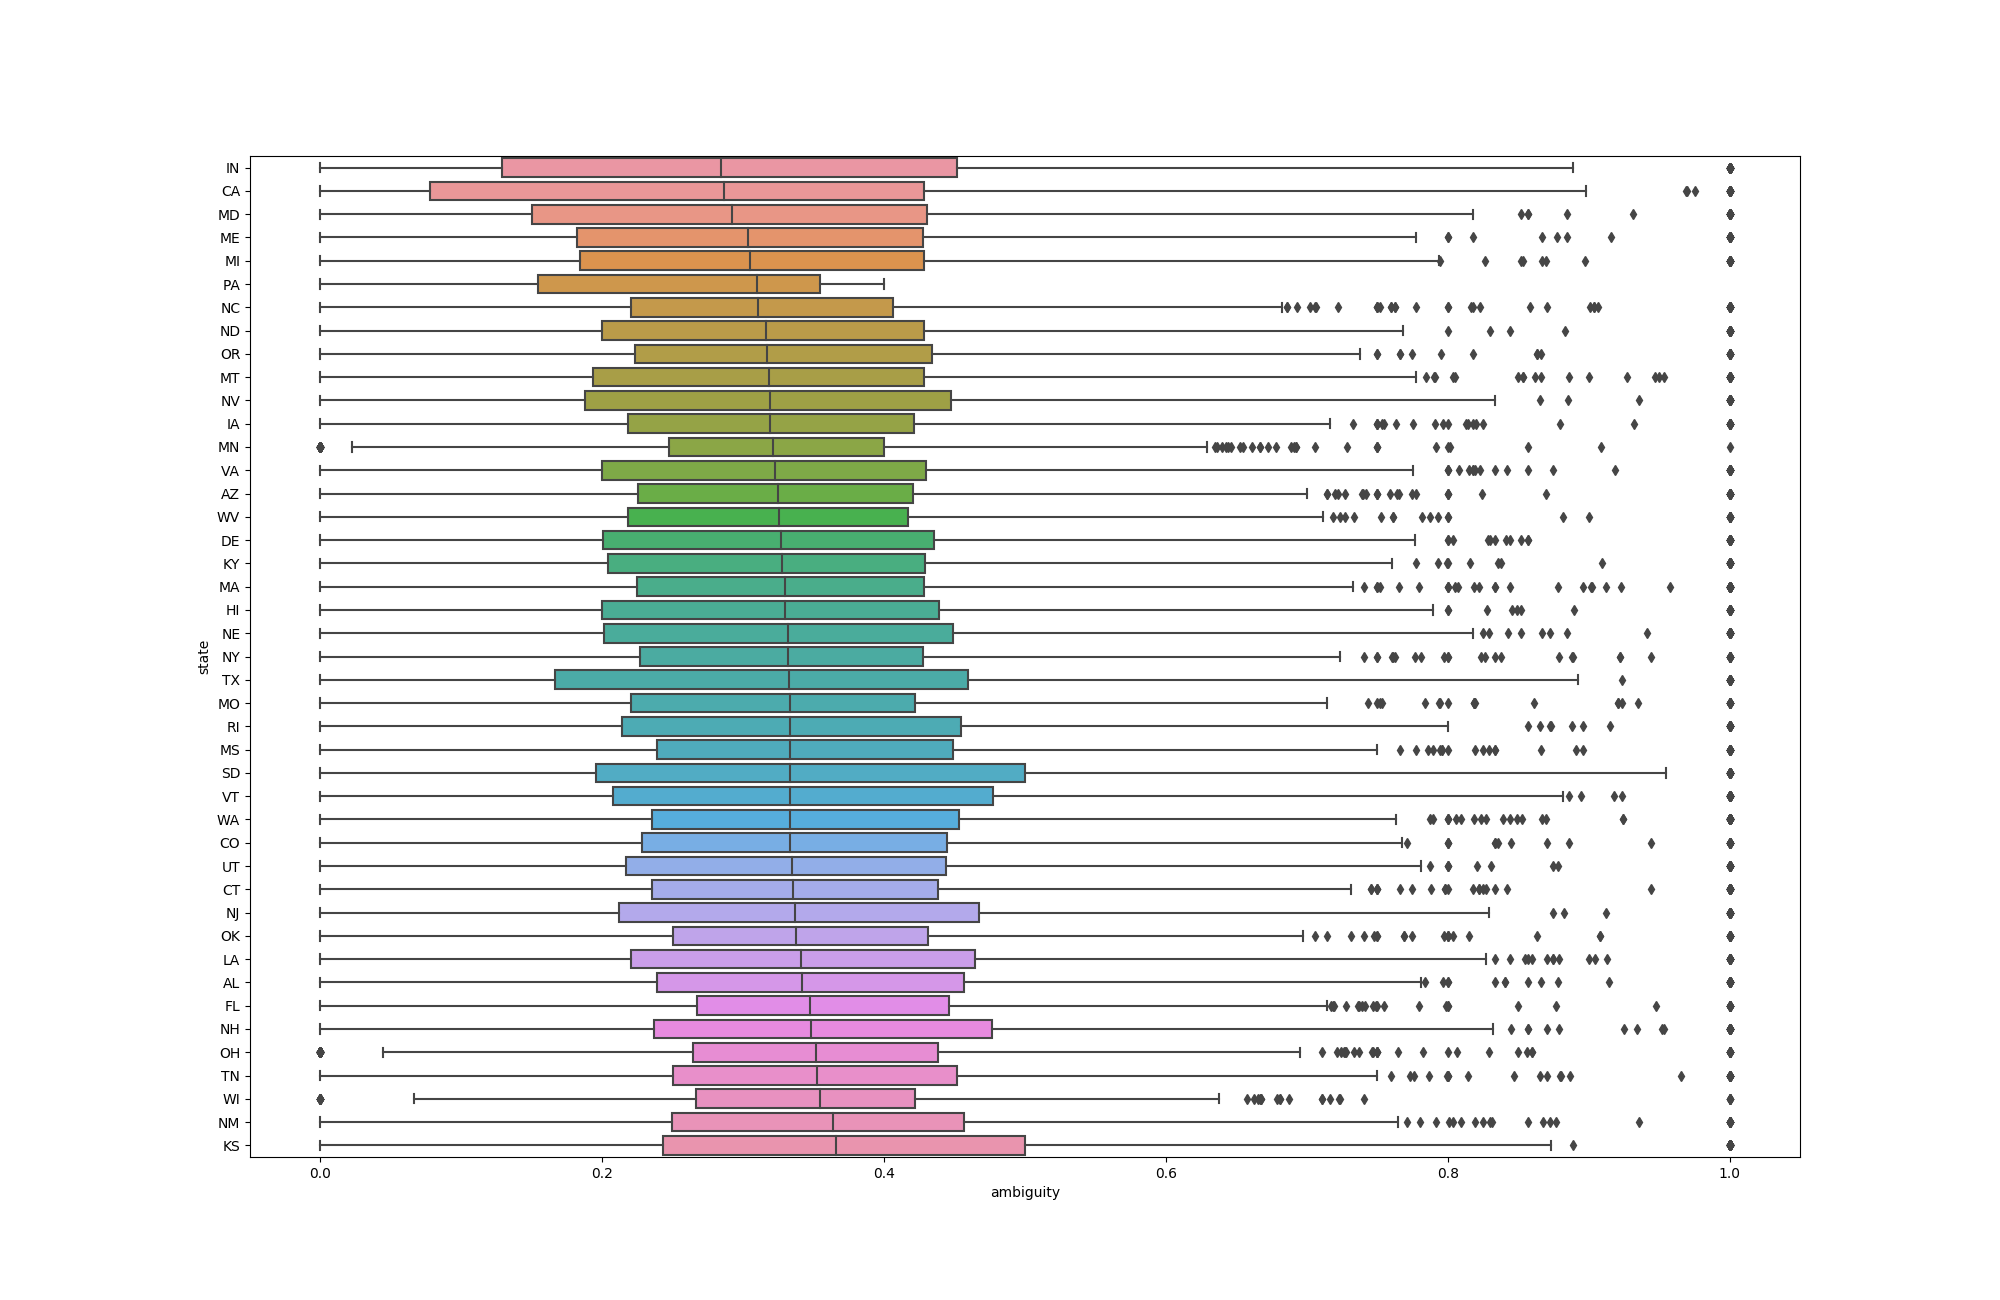
\includegraphics[width=14cm]{images/uss_ambiguity_by_state.png}
\end{center}
\caption{Accumulated distribution of ambiguity scores by state}
\label{fig:uss_ambiguity_by_state}
\end{figure}


In fact the correlation (Pearson correlation coefficient, $[-1, +1]$) between the state's averaged campaign contribution limit and the accumulated ambiguity score is slightly negative, i.e. increasing ambiguity with decreasing contribution limits. However, the correlation efficient is not very large, compared to the correlation between the campaign contribution limits and other text features such as the number of numerical values. These are about six times stronger (linearly) correlated than the determined ambiguity score. Surprisingly, the number of tokens are inversely correlated, having a positive correlation coefficient. 

\begin{figure}[h!]
\begin{center}
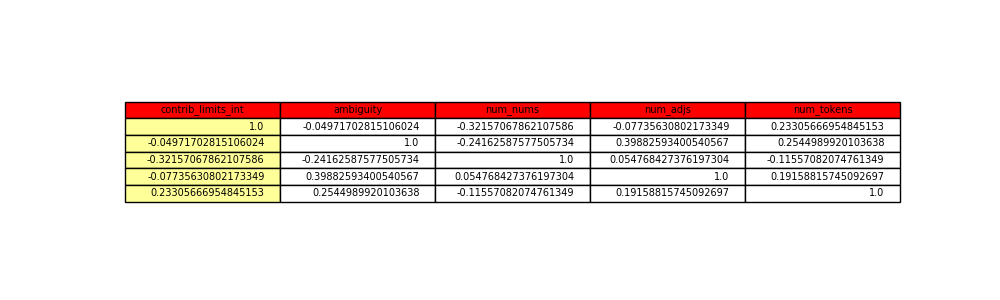
\includegraphics[width=14cm]{images/correlation_table.png}
\end{center}
\caption{Correlation matrix between campaign contribution limits, ambiguity score and text features}
\label{fig:correlation_table}
\end{figure}

Figure \ref{fig:uss_ambiguity_by_sector} shows the accumulated ambiguity scores over the separated industry sectors, whereas bills that could not be assigned to one of the sectors are classified as \textit{other}. Similar to the states the ambiguity scores do not differ a lot from one industry sector to another. An overall analysis over all states and sectors can be found in the appendix. 

\begin{figure}[h!]
\begin{center}
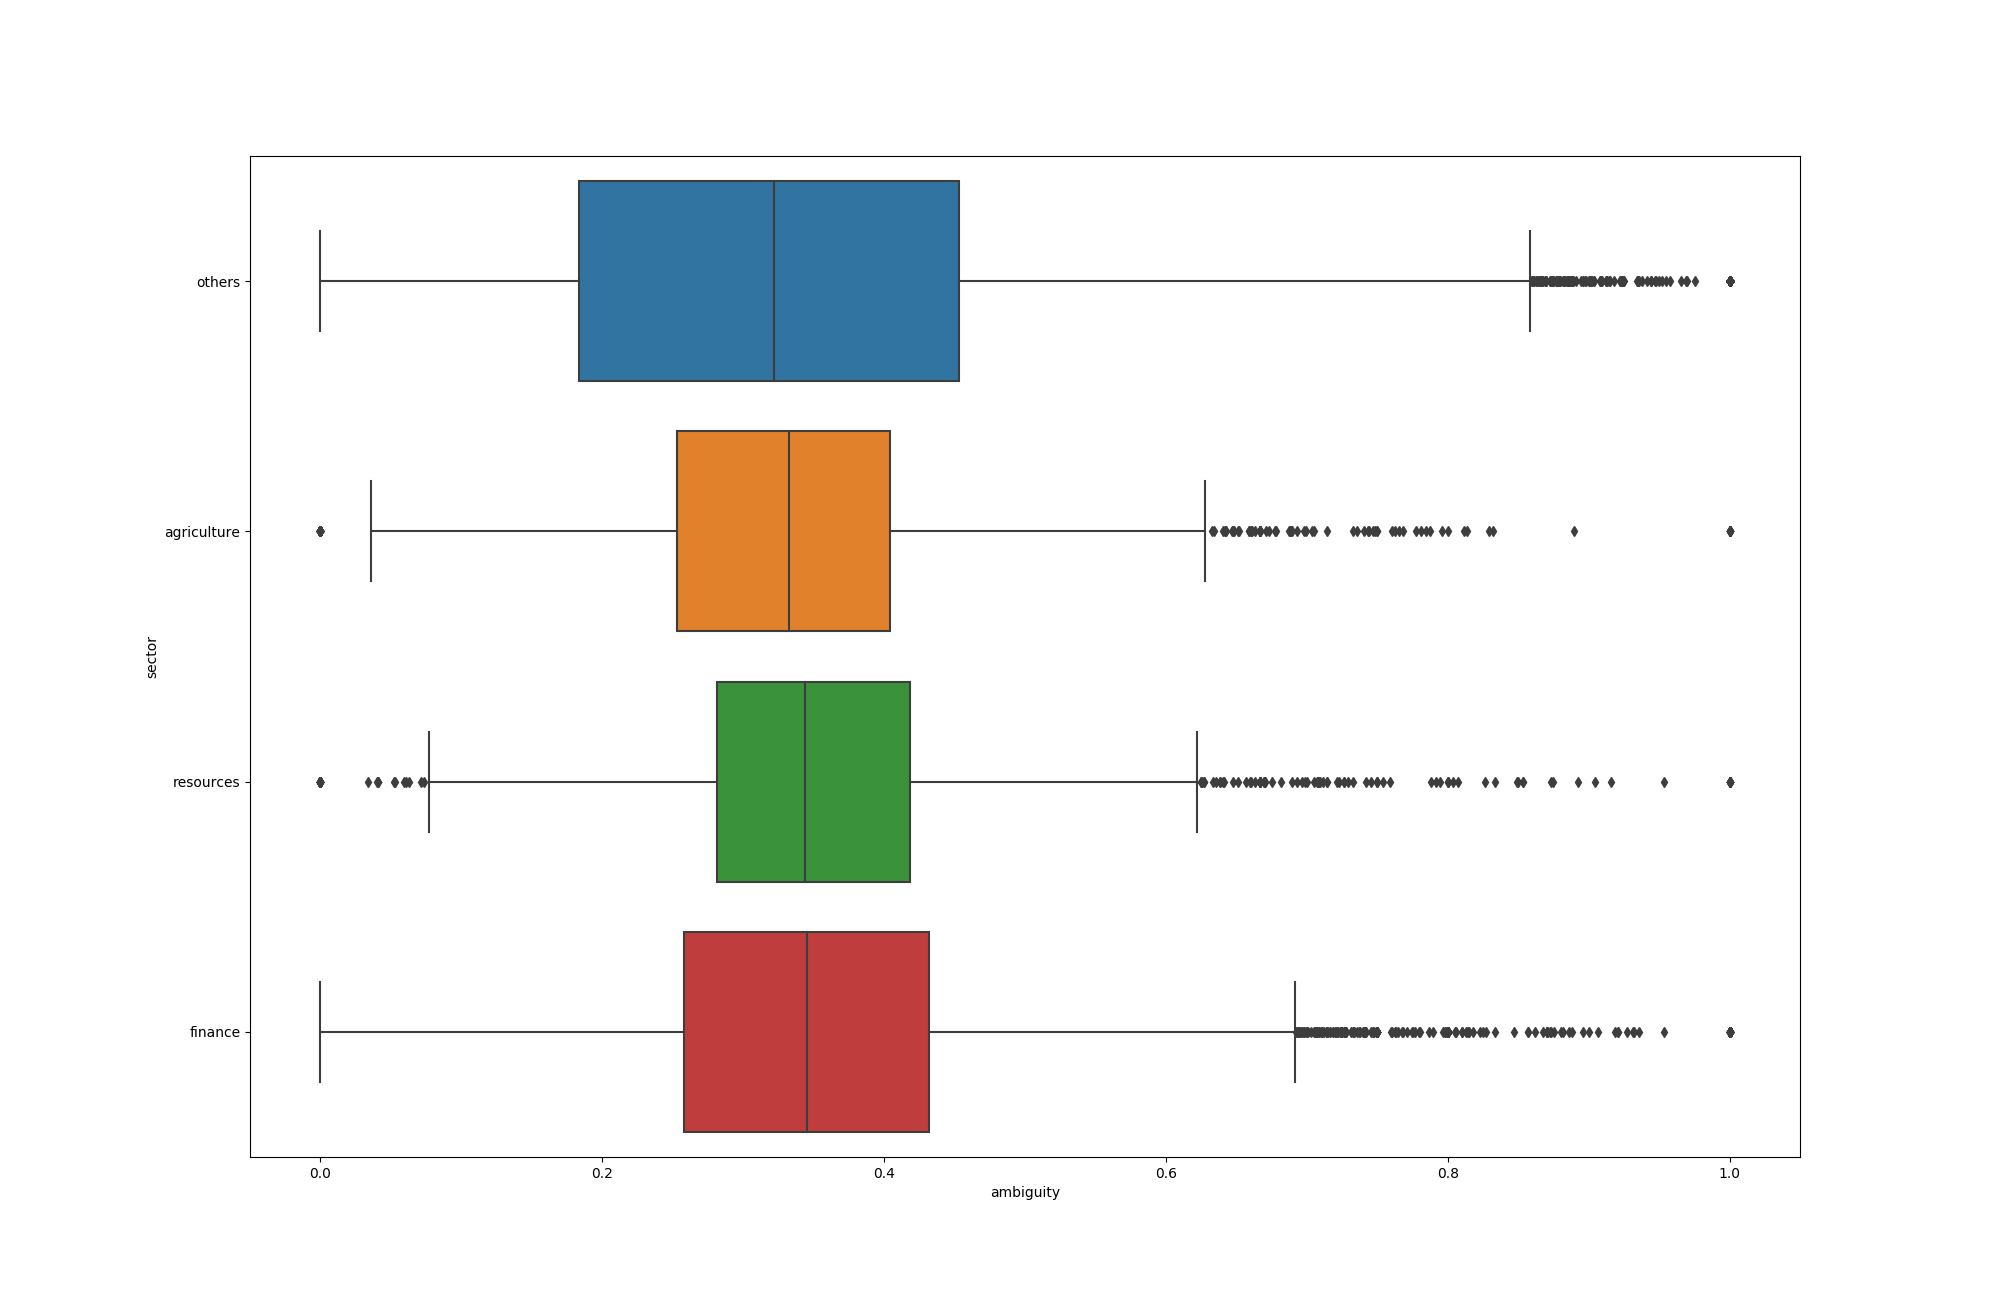
\includegraphics[width=10cm]{images/uss_ambiguity_by_sector.png}
\end{center}
\caption{Accumulated distribution of ambiguity scores by industry sector}
\label{fig:uss_ambiguity_by_sector}
\end{figure}

%=================================================================================
% CONCLUSION and FUTURE WORK
%=================================================================================
\chapter{Conclusion}
\label{cha:conclusion}
Within this project the impact of campaign contributions on the ambiguity of bills has been analyzed at the example of US states bills. As shown there is a correlation between the accumulated ambiguity of adopted bills in US states in the period of 1950 to 1999 and the state's campaign contribution limits in an anti-proportional manner, i.e. the more restricted the campaign contribution limits are, overall the less ambiguous the bills are. However this correlation is not very large, compared to other text features. Also, as described, the accumulated ambiguity does not vary much over several industry sectors. 
\newline
This work leaves several avenues for future work. Firstly, the dictionary based topic modelling approach was chosen for efficiency reasons, taking into account the large amount of text data being processed, however more advanced topic modelling methods (e.g. using Latent Dirichlet Allocation \cite{lda_topic_modeling} or Word2Vec \cite{word2vec}) could be used instead and the number of sector clusters could be increased. Similarly the word-sense and similarity based ambiguity evaluation that was used in this project is very efficient and works for general text data, but also is limited by the complexity of the underlying sense taxonomy. Going further an unsupervised learning algorithm could be used, such as the page rank algorithm purposed in \cite{knowledge_based_page_rank}, to apply word-sense-disambiguation on a database specifically trained on law text data. Thirdly, in order to differentiate the impact of different sectors on the bill's ambiguity external, state-dependent factors have be excluded (multiple comparison problem). Besides, during evaluation the ambiguity have been accumulated over several years, mainly due to the leak of computational resources. Although as shown in Figure \ref{fig:usc_grid} the contribution limits do not change much over time, time-dependent effects have been excluded here. In further work external, state-dependent effects as well as time-dependent effects, maybe due to changes in government, financial crises, etc. could be taken into account. Also due to the datasets used not the actual, sector-splitted campaign contributions have been taken into account but the contribution limits, while a uniform contribution distribution over the industry sectors has been assumed. In further work the actual campaign contributions can be separated by industry sector. 

%=================================================================================
% BIBLIOGRAPHY
%=================================================================================
\bibliographystyle{plain}
% Force the bibliography not to be numbered
% \renewcommand{\thechapter}{0}
\bibliography{references}

%=================================================================================
% APPENDIX
%=================================================================================
\section*{Appendix - Ambiguity scores by state and industry sector}
\centerline{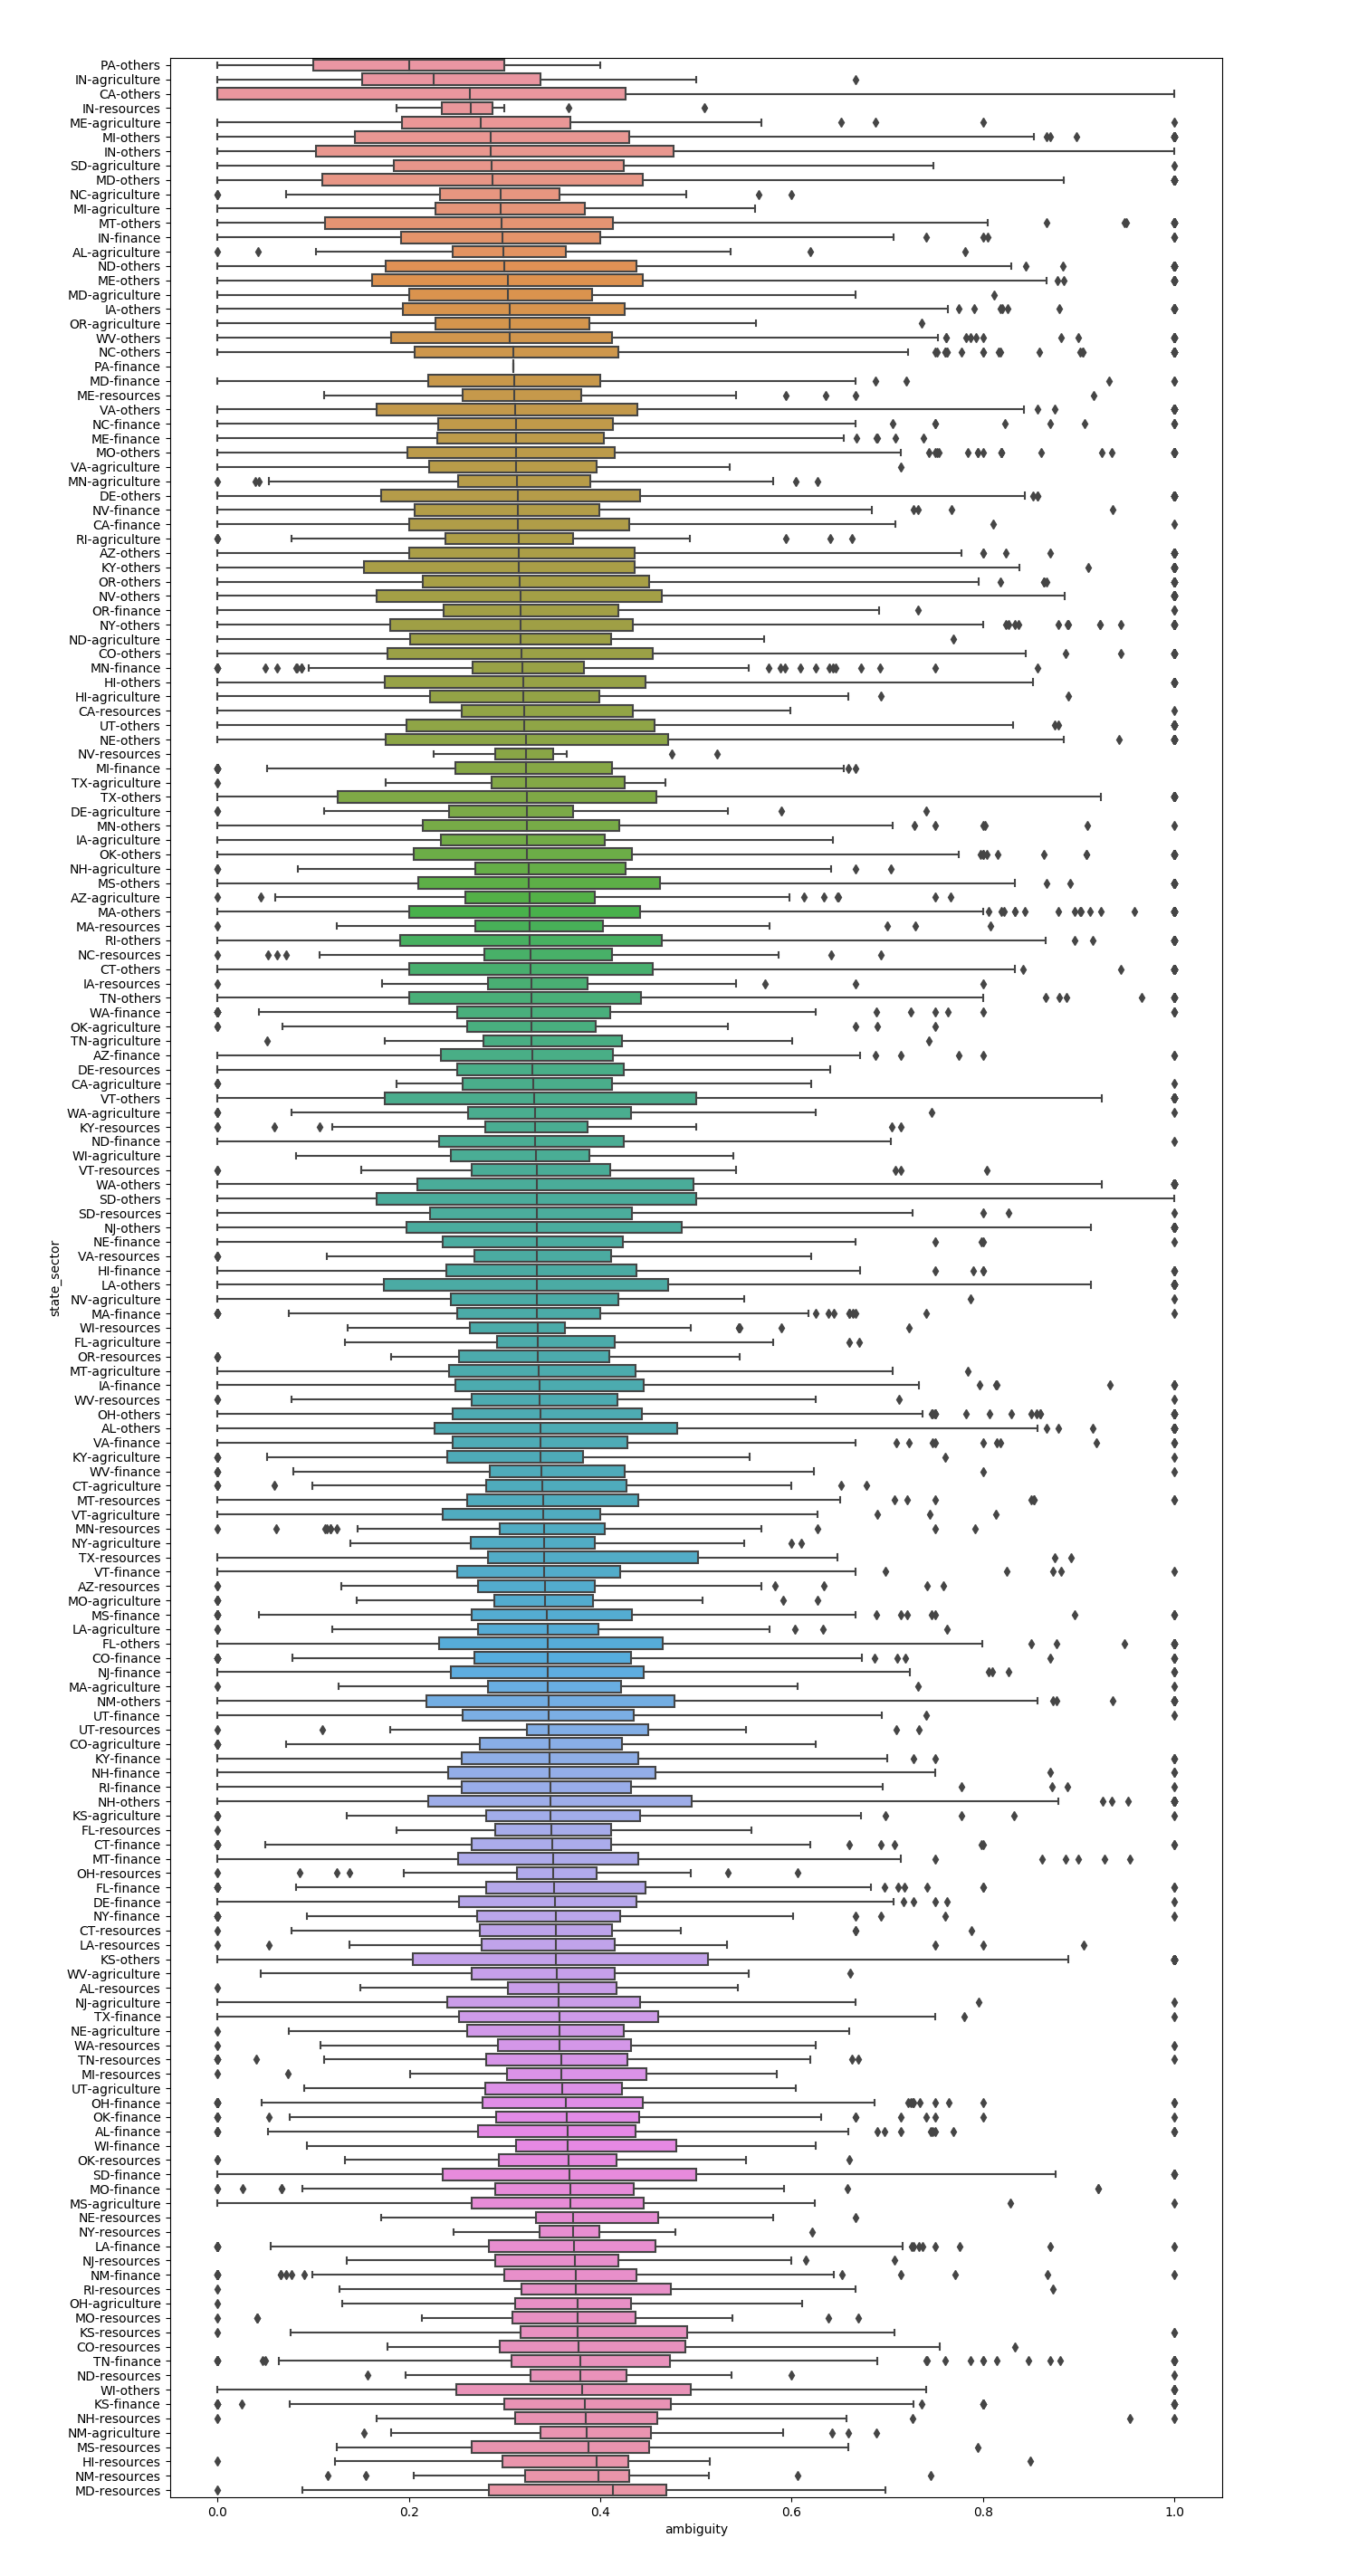
\includegraphics[width=12cm]{images/uss_ambiguity_state_sector.png}}

\section*{Appendix - Campaign contribution limits and accumulated ambiguity scores by state in US map}
\centerline{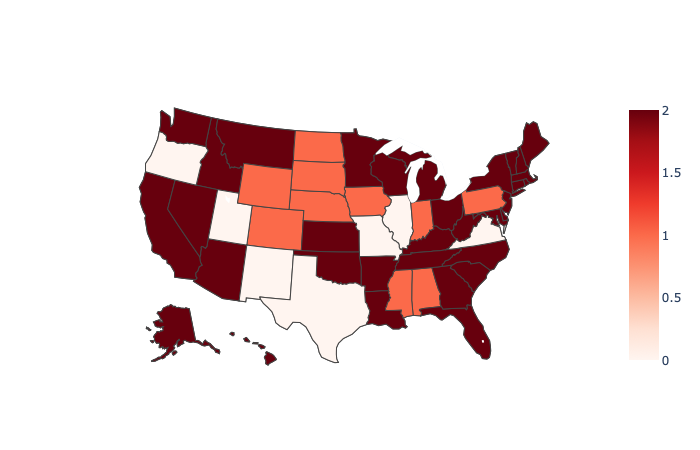
\includegraphics[width=14cm]{images/usc_map.png}}
\centerline{Campaign contribution limits: 0 = \textit{unlimited}, 1 = \textit{individual}, 2 = \textit{restricted} in 1999}
\centerline{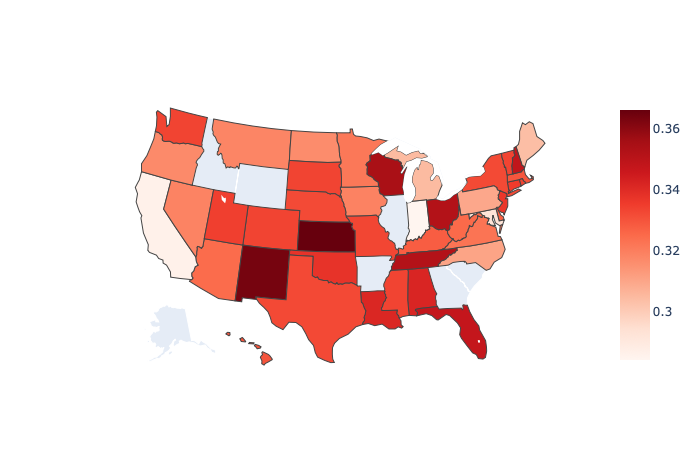
\includegraphics[width=14cm]{images/uss_ambiguity_map.png}}
\centerline{Accumulated ambiguity scores: 0 = \textit{un-ambiguous}, 1 = \textit{very ambiguous} }

\end{document}
